\documentclass[compress,red]{beamer}
\usepackage[utf8]{inputenc}
\usepackage{ucs}
\usepackage{amsmath}
\usepackage{amsfonts}
\usepackage{amssymb}
\usepackage[russian]{babel}
\usepackage{graphicx}
\usepackage{wrapfig}

\usepackage{tikz}
\usepackage{verbatim}

\usepackage{color}
\usepackage{xcolor}
\usepackage{listings}

\usepackage{caption}

\lstset{
language=ruby,
extendedchars=\true,
inputencoding=utf8x,
commentstyle=\itshape,
stringstyle=\bf,
belowcaptionskip=5pt }


\DeclareCaptionFont{white}{\color{white}}
\DeclareCaptionFormat{listing}{\colorbox{gray}{\parbox{\textwidth}{#1#2#3}}}
\captionsetup[lstlisting]{format=listing,labelfont=white,textfont=white}

\usetikzlibrary{calc,trees,positioning,arrows,chains,shapes.geometric,%
    decorations.pathreplacing,decorations.pathmorphing,shapes,%
    matrix,shapes.symbols}

\tikzset{
>=stealth',
  punktchain/.style={
    rectangle, 
    rounded corners, 
    % fill=black!10,
    draw=black, very thick,
    text width=10em, 
    minimum height=3em, 
    text centered, 
    on chain},
  line/.style={draw, thick, <-},
  element/.style={
    tape,
    top color=white,
    bottom color=blue!50!black!60!,
    minimum width=8em,
    draw=blue!40!black!90, very thick,
    text width=10em, 
    minimum height=1.5em, 
    text centered, 
    on chain},
  every join/.style={->, thick,shorten <=1pt},
  decoration={brace},
  tuborg/.style={decorate},
  tubnode/.style={midway, right=2pt},
}

\mode<presentation>

\usetheme{Warsaw}

\definecolor{Red}{rgb}{1,0,0}
\definecolor{Blue}{rgb}{0,0,1}
\definecolor{Green}{rgb}{0,1,0}
\definecolor{magenta}{rgb}{1,0,.6}
\definecolor{lightblue}{rgb}{0,.5,1}
\definecolor{lightpurple}{rgb}{.6,.4,1}
\definecolor{gold}{rgb}{.6,.5,0}
\definecolor{orange}{rgb}{1,0.4,0}
\definecolor{hotpink}{rgb}{1,0,0.5}
\definecolor{newcolor2}{rgb}{.5,.3,.5}
\definecolor{newcolor}{rgb}{0,.3,1}
\definecolor{newcolor3}{rgb}{1,0,.35}
\definecolor{darkgreen1}{rgb}{0, .35, 0}
\definecolor{darkgreen}{rgb}{0, .6, 0}
\definecolor{darkred}{rgb}{.75,0,0}

\xdefinecolor{olive}{cmyk}{0.64,0,0.95,0.4}
\xdefinecolor{purpleish}{cmyk}{0.75,0.75,0,0}

\useoutertheme[subsection=false]{smoothbars}

\title{Логические уравнения}

%\usecolortheme{dolphin}


\begin{document}
%%титульная страница
\maketitle
%% основные моменты

\section{Повторение}

\subsection{Повторение}
\begin{frame}[fragile]
  \frametitle{Повторим основные операции}
  \begin{center}
    \Huge{$\neg$}
  \end{center}
  \begin{center}
    \Huge{$\&$}
  \end{center}
  \begin{center}
    \Huge{$\vee$}
  \end{center}
\end{frame}

\subsection{Повторение таблицы истинности}
\begin{frame}
    \frametitle{Повторим таблицы истинности}
    \begin{columns}[c]
        \column{.3\textwidth}
            \begin{center}
              \begin{tabular}{|c|c|c|}
                \hline
                A & B & A \& B \\
                \hline
                И & И & И \\
                \hline
                И & Л & Л \\
                \hline
                Л & И & Л \\
                \hline
                Л & Л & Л \\
                \hline
              \end{tabular}
            \end{center}
            
        \column{.3\textwidth}
            \begin{center}
                \begin{tabular}{|c|c|c|}
                    \hline
                    A & B & $A \vee B$ \\
                    \hline
                    И & И & И \\
                    \hline
                    И & Л & И \\
                    \hline
                    Л & И & И \\
                    \hline
                    Л & Л & Л \\
                    \hline
                \end{tabular}
            \end{center}

        \column{.3\textwidth}
            \begin{center}
              \begin{tabular}{|c|c|}
                \hline
                A & ${\neg} A$ \\
                \hline
                И & Л \\
                \hline
                Л & И \\
                \hline
              \end{tabular}
            \end{center}
    \end{columns}                        
\end{frame}

\subsection{Пара задач}
\begin{frame}[fragile]
  \frametitle{Проверим знание}
  \begin{itemize}[<+->]
    \item<1->И \& (И $\vee$ Л ) = \only<2->{И}
    \item<3->И $\vee$ Л \& И = \only<4->{И}
    \item<5->${\neg}$ И \& ${\neg}$Л $\vee$ Л = \only<6->{Л}
    \item<7->${\neg}$ И $\vee$ (${\neg}$Л $\vee$ Л \& И) = \only<8->{И}
    \item 
  \end{itemize}
\end{frame}

\subsection{Правила де Моргана}
\begin{frame}[fragile]
  \frametitle{Вспомним правила Де Моргана}
  
  \begin{itemize}
      \item
      \begin{tabular}{|l|l|l|}
        \hline
        Правила де Моргана & ${\neg}$(A$\&$B) = ${\neg}$A$\vee$${\neg}$B \\
                           & ${\neg}$(A$\vee$B) = ${\neg}$A$\&$${\neg}$B \\
        \hline
      \end{tabular}
    \item<1->${\neg}$A \& ${\neg}$(${\neg}$B $\vee$ C) = \only<2->{${\neg}$A \& (${\neg}$${\neg}$B \& ${\neg}$C) =}\only<3->{${\neg}$A \& B \& ${\neg}$C}
    \item<4->${\neg}$(A $\vee$ ${\neg}$(${\neg}$B $\vee$ C) = \only<5->{${\neg}$A $\&$ ${\neg}$${\neg}$(${\neg}$B $\vee$ C) = }\only<6->{${\neg}$A \& (${\neg}$B $\vee$ C) =}
    \item<7-> Вспомним распределительный закон:
    
        \begin{tabular}{|l|l|l|}
          \hline
          Распределительный & A$\&$(B$\vee$C)~=~(A$\&$B)$\vee$(A$\&$C) \\
                        & A$\vee$(B$\&$C)~=~(A$\vee$B)$\&$(A$\vee$C) \\
          \hline
        \end{tabular}
        
    }
    \item<8->(${\neg}$A \& ${\neg}$B) $\vee$ (${\neg}$A \& C) = \only<9->{${\neg}$A \& ${\neg}$B $\vee$ ${\neg}$A \& C}
  \end{itemize}
\end{frame}

\section{ЕГЭ}

\subsection{Задачи из ЕГЭ}
\begin{frame}[fragile]
  \frametitle{ЕГЭ: правила де Моргана}
  \begin{itemize}
      \item<1->Считая, что за символ $\wedge$ обозначается конъюнкция, вычислите правильный ответ.
      \item<2->Правильный ответ: 1
  \end{itemize}
  \centerline{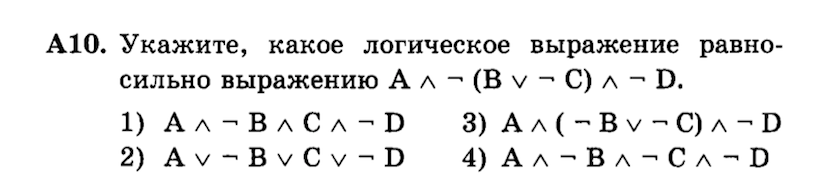
\includegraphics[width=0.8\textwidth]{images/logic-01.png}}
\end{frame}

\subsection{Задачи из ЕГЭ 2}
\begin{frame}[fragile]
  \frametitle{ЕГЭ: правила де Моргана}
  \begin{itemize}
      \item<1->Считая, что за символ $\wedge$ обозначается конъюнкция, вычислите правильный ответ.
      \item<2->Правильный ответ: 3
  \end{itemize}
  \centerline{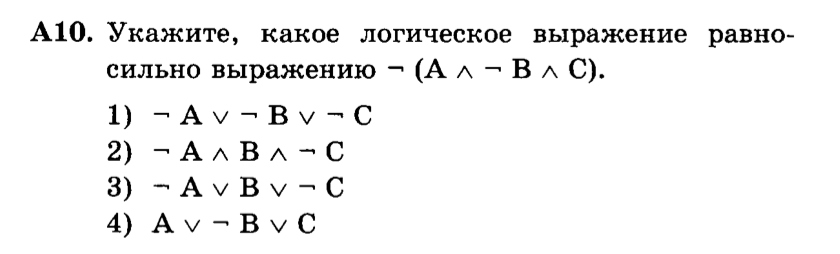
\includegraphics[width=0.8\textwidth]{images/logic-02.png}}
\end{frame}

\subsection{Таблица истинности}
\begin{frame}[fragile]
  \frametitle{ЕГЭ: таблицы истинности}
  \begin{itemize}
      \item \small{Считая, что за символ $\wedge$ обозначается конъюнкция, 1 --- истина, 0 --- ложь, вычислите правильный ответ.}
  \end{itemize}
  \centerline{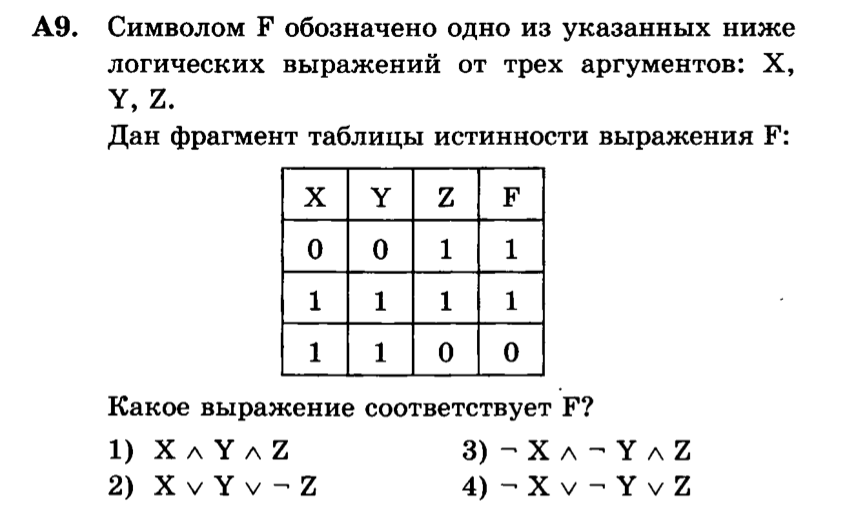
\includegraphics[width=0.6\textwidth]{images/logic-04.png}}
\end{frame}

\subsection{Решение таблицы истинности}
\begin{frame}[fragile]
  \frametitle{ЕГЭ: решение задачи}
  \begin{itemize}
    \item Рассмотрим 1-ый вариант и подставим его в таблицу. 
        \begin{enumerate}
            \item Если для всех трёх строк он подойдёт, то этот ответ и будет являться правильным. 
            \item Если хотя бы для одной строки 1-ый ответ не подходит, следовательно, это --- неправильный ответ. В этом случае мы переходим ко второму варианту.
        \end{enumerate}
    \item Подставим 1-ый вариант в 1-ую строку:
    \item Л \& Л \& И должно равняться (согласно таблице) Истине. 
    \item Однако: Л \& Л \& И = Л \& И = Л.
    \item Таким образом, получаем противоречие. Следовательно, первый ответ заведомо неверный.
    \item Аналогично находим, что второй ответ не подходит к третьей строке, третий ответ не подходит ко второй строке. Следовательно, остаётся четвёртый.
    \item Подстановкой убеждаемся, что 4-ый ответ подходит во все строки.
  \end{itemize}
\end{frame}

\subsection{Таблица истинности 2}
\begin{frame}[fragile]
  \frametitle{Задача 2 на таблицу истинности}
  \centerline{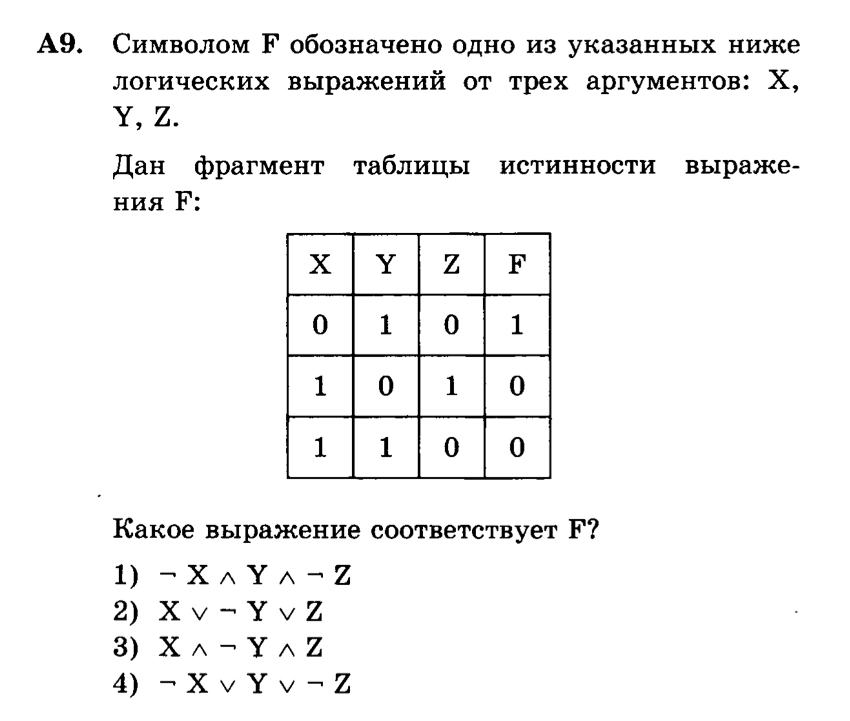
\includegraphics[width=0.8\textwidth]{images/logic-03.png}}
\end{frame}

\subsection{Импликация}
\begin{frame}
  \begin{center}
    \Huge{Импликация}
  \end{center}
\end{frame}

\subsection{Таблица истинности для конъюнкции}
\begin{frame}[fragile]
  \frametitle{Таблица истинности для конъюнкции}
  \begin{itemize}
    \item \emph{Импликация} --- ещё одна логическая операция, которая расшифровывается как \emph{следовательно}.
    \item Обозначение: A $=>$ B. Выполняется \textbf{после} всех основных операций.
  \end{itemize}
  \begin{center}
    \begin{tabular}{|c|c|c|}
      \hline
      A & B & A => B \\
      \hline
      И & И & И \\
      \hline
      И & Л & Л \\
      \hline
      Л & И & И \\
      \hline
      Л & Л & И \\
      \hline
    \end{tabular}
  \end{center}
\end{frame}

\subsection{Правило}
\begin{frame}
  \begin{center}
    \Huge{Правило импликации}
  \end{center}
  \begin{center}
    \Large{Из лжи может следовать всё, что угодно.}
  \end{center}
\end{frame}

\subsection{Пример импликации}
\begin{frame}
  \begin{center}
    \Large{\{И \& И => Л\} = \{И => Л = Л\}}
  \end{center}
\end{frame}

\subsection{Задача на импликацию}
\begin{frame}[fragile]
  \frametitle{Задача на импликацию}
  \begin{itemize}[<+->]
    \item Найти максимальное целое X, при котором истинно высказывание:
        \begin{itemize}
            \item $(90 < X\cdot X) => (X < (X-1))$
        \end{itemize}
    \item \textbf{Решение:} Рассмотрим внимательно правую часть. Она всегда ложна, так как X всегда больше $X-1$.
    \item Следовательно, левая часть обязана быть тоже ложной, так как если бы она была истинной, то всё высказывание бы стало ложным (И=>Л=Л).
    \item До каких пор 90 больше $X^2$?
    \item До 9 включительно, так как $10^2 = 100 > 90$.
    \item При $X\geq 10$ левая часть станет истинной, а высказывание станет ложным.
    \item Следовательно, \textbf{ответ}: $X = 9$.
  \end{itemize}
\end{frame}

\subsection{Задачи на импликацию}
\begin{frame}[fragile]
  \frametitle{Задачи на импликацию}
  \begin{enumerate}
    \item Найдите максимальное положительное целое число $X$, при котором \textbf{истинно} высказывание:
        \begin{itemize}
            \item $((X - 1) < X) => (40 > X\cdot X)$
        \end{itemize}
    \item Найдите наименьшее целое положительное число $X$, при котором \textbf{ложно} высказывание:
         \begin{itemize}
             \item ${\neg}(X\cdot X < 9) => (X >(X + 2))$
         \end{itemize}
    \item Найдите наименьшее целое положительное число $X$, при котором \textbf{ложно} высказывание:
        \begin{itemize}
            \item $(4 > -(4 + X)\cdot X)) => (30 > X\cdot X)$
        \end{itemize}
  \end{enumerate}
\end{frame}

\end{document}